%-*-latex-*-
\input{myquizpreamble.tex}
\input{ciss240.tex}
\input{yliow}
\renewcommand\TITLE{Quiz q0102}

\begin{document}
\topmatter

FOR SPRING2022: Because we are meeting virtually and also because
the college has discouraged passing around printouts,
open any text editor (example: notepad), write the corrected program
named \verb!main.cpp!,
email \verb!yliow@ccis.edu! using your college email account with
subject line \lq\lq \verb!ciss240 q0102!", attach your main.cpp.
You should NOT use your C++ compiler (MSVS, etc.) to test your \verb!main.cpp!.

This is NOT an open book quiz. 
You have 3 minutes. 

Q1. The goal is correct a C++ program by hand without the help of a C++ 
compiler software.
\begin{tightlist}
\li To delete something: cross it out clearly.
\li To insert something: draw a box,
      put whatever you want to insert into the box, and draw an arrow
      from the box to the point where you want to insert to go.
\li To modify something: do a delete and an insert.
\end{tightlist}
For instance
\begin{center}
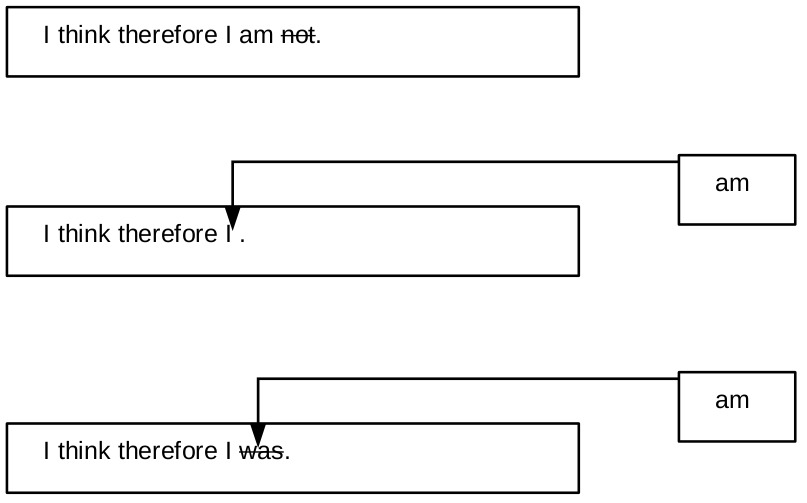
\includegraphics[width=5in]{q01-02.jpg}
\end{center}


Write clearly and legibly. If I cannot read what you wrote, you will get zero. 

TURN THE PAGE FOR THE PROGRAM TO CORRECT.

\newpage

Correct the following program. The intended output is given below.



PROGRAM:
{\Large
\begin{console}


#include iostream

int Main()
(
    std::cout >> '2b or not 2b'

    return 0
)


\end{console}
}



INTENDED OUTPUT:
\begin{console}
2b or not 2b
\end{console}

\textsc{Grading}:
\begin{tightlist}
\li Each correct deletion/insertion/modification is worth 1 point.
\li Each incorrect deletion/insertion/modification is worth -1 point.
\li Your total is normalized to 3 points. 
(I'm not telling you the total number of corrections.)
\end{tightlist}
\end{document}
